\documentclass[reqno,11pt]{amsart}
\usepackage[utf8x]{inputenc}
\usepackage{xcolor}
\usepackage{amssymb}
\usepackage{amsmath}
\usepackage[T1]{fontenc}
\usepackage{tikz}
\usetikzlibrary{quotes,angles}

\begin{document}

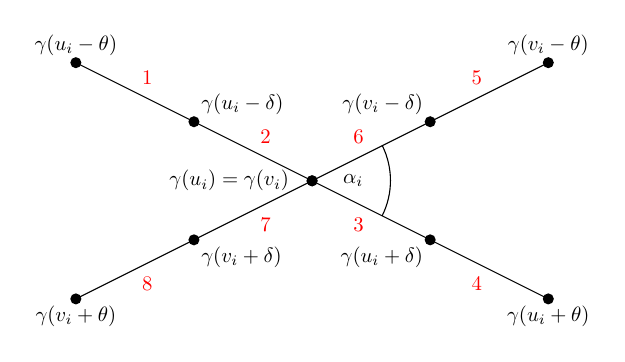
\begin{tikzpicture}
\draw[-] (-3,1.5) -- (-1.5,0.75);
\draw[-] (-1.5,0.75) -- (0,0);
\draw[-] (0,0) -- (1.5,-0.75);
\draw[-] (1.5,-0.75) -- (3,-1.5);
\draw[-] (-3,-1.5) -- (-1.5,-0.75);
\draw[-] (-1.5,-0.75) -- (0,0);
\draw[-] (0,0) -- (1.5,0.75);
\draw[-] (1.5,0.75) -- (3,1.5);
\draw (-2.25,1.125) node[red,above right,scale=0.75] {$1$};
\draw (-0.75,0.375) node[red,above right,scale=0.75] {$2$};
\draw (0.75,-0.375) node[red,below left,scale=0.75] {$3$};
\draw (2.25,-1.125) node[red,below left,scale=0.75] {$4$};
\draw (2.25,1.125) node[red,above left,scale=0.75] {$5$};
\draw (0.75,0.375) node[red,above left,scale=0.75] {$6$};
\draw (-0.75,-0.375) node[red,below right,scale=0.75] {$7$};
\draw (-2.25,-1.125) node[red,below right,scale=0.75] {$8$};
\draw[black] (0.89,0.45) arc (26.57:-26.57:1);
\draw (0.3,0) node[black,right,scale=0.75] {$\alpha_i$};
\draw (-3,1.5) node[black,above,scale=0.75] {$\gamma(u_i-\theta)$};
\draw (3,-1.5) node[black,below,scale=0.75] {$\gamma(u_i+\theta)$};
\draw (-3,-1.5) node[black,below,scale=0.75] {$\gamma(v_i+\theta)$};
\draw (3,1.5) node[black,above,scale=0.75] {$\gamma(v_i-\theta)$};
  \draw (-1.5,0.75) node[black,above right,scale=0.75] {$\gamma(u_i-\delta)$};
\draw (1.5,-0.75) node[black,below left,scale=0.75] {$\gamma(u_i+\delta)$};
\draw (-1.5,-0.75) node[black,below right,scale=0.75] {$\gamma(v_i+\delta)$};
\draw (1.5,0.75) node[black,above left,scale=0.75] {$\gamma(v_i-\delta)$};
\fill[black] (-3,1.5) circle (2pt);
\fill[black] (-3,-1.5) circle (2pt);
\fill[black] (3,1.5) circle (2pt);
\fill[black] (3,-1.5) circle (2pt);
\fill[black] (0,0) circle (2pt);
\fill[black] (-1.5,0.75) circle (2pt);
\fill[black] (-1.5,-0.75) circle (2pt);
\fill[black] (1.5,0.75) circle (2pt);
\fill[black] (1.5,-0.75) circle (2pt);
\fill[black] (0,0) circle (2pt);
\draw (-0.2,0) node[black,left,scale=0.75] {$\gamma(u_i)=\gamma(v_i)$};
\end{tikzpicture}

\end{document}